\section{Introduction}

Space is a growing industry with thousands of satellites in orbit currently and, with the introduction of satellite constellations, thousands more to come in the next decades. In this context automation of is key importance to keeping costs down. The attitude determination and control system (ACDS) enables a satellite to orient itself and is thus critical for operations such as communication and observation. Due to the inaccessible nature of orbit, fault-tolerant control (FTC) is an attractive method of allowing operations to continue after degradation or even failure of an actuator. Current industry standard methods of dealing with this problem involve putting the satellite into safe mode and solving the problem on the ground. This paper proposes to solve this problem online automatically using a fault detection and isolation unit (FDI) and an FTC unit.

\section{Problem Definition}

\section{Literature Review}

\subsection{Satellite Attitude Kinematics}

\subsubsection{Attitude representations}
The satellite's orientation can be represented intuitively using euler angles such as yaw $\psi$, pitch $\theta$ and roll$\phi$. However these representations are not so effective for computation in attitude control as they require more expensive trigonometric functions to be used and produce singularities. The most accurate way to represent the attitude of an object is using the direction cosine matrix (DCM) aka. the rotation matrix. This is a 3x3 matrix where each column represents the orthogonal xyz axes vector. However this is cumbersome for computing calculations as it would require computing 9 differential equations to determine a satellite's attitude. Instead quaternions are used during computations. The quaternion can be defined as: 

\begin{equation}
    \begin{bmatrix}
        q_{1} \\ q_{2} \\ q_{3} \\ q_{4}
    \end{bmatrix}
    =
    \begin{bmatrix}
        e_{1}\sin(\Phi) \\ e_{2}\sin(\Phi) \\ e_{3}\sin(\Phi) \\ q_{4}\cos(\Phi)
    \end{bmatrix}
\end{equation}



\subsection{Attitude Control of a Satellite}
\subsubsection{Dynamics and Kinematics}
The attitude of a vehicle refers to it's orientation and angular rate in 3D space. In order to control a satellite's oritentation for pointing and other applications it's dynamics and kinemeatics must be understood and modelled. The motion of a satellite can be described by the kinematic equation \cite{sidiAttitudeDynamicsKinematics1997}:
\begin{equation}
    \vec{\dot{Q}}
=\frac{1}{2}
\begin{bmatrix}
q_{0} \ \ \neg q_{3} \ \ \ q_{2} \\ 
q_{3} \ \ q_{0} \ \ \ \neg q_{1} \\ 
\neg q_{2} \ \ q_{1} \ \ \ q_{0} \\ 
\neg q_{1} \ \ \neg q_{2} \ \ \ \neg q_{3} \\
\end{bmatrix} \vec{\omega_{b}}
\end{equation}

where $\vec{\omega_{b}}$ is the satellite's angular rate vector and $\vec{Q}$ is the quaternion representation of the satellite's attitude. 

A satellite's attitude with mass moment of inertia $\boldsymbol{J}$ can be modelled using the Newton-Euler equation \cite{sidiAttitudeDynamicsKinematics1997}: 

\begin{equation}
\mathbf{J}\mathbf{\dot{\vec{\omega}}_b} = \sum{\mathbf{T_{ext}}} -\mathbf{\vec{\omega_{b}}}\times(\mathbf{J}\vec{\omega_{b}}-\vec{h})-\vec{\dot{h}}
\end{equation}

where $\boldsymbol{\vec{\omega_{b}}}$ is the satellite's angular rate vector, $\boldsymbol{T_{ext}}$ is any external torque applied

\subsection{Quaternion Feedback Control}
A common control law designed used for 3-axis pointing control is the quaternion feedback control law. It uses proportional and derivative control to output a control signal $\vec{u}$ and is given by \cite{wieSpaceVehicleDynamics1998}:

\begin{equation}
    \vec{u} = -\vec{K_{q}}\vec{q_{e}} - \vec{K_{\omega}}\vec{\omega_{e}}
\end{equation}

where $\vec{K_{q}}$ and $\vec{K_{\omega_{b}}}$ are the quaternion and angular rate feedback gains respectively and $\vec{q_{e}}$ and $\vec{\omega_{e}}$ 
are the quaternion and angular rate errors respectively.

\subsection{Fault Detection and Isolation}
Fault detection and isolation (FDI) is crucial for providing up to date fault information for controller reconfiguration. In literature FDI is commonly used however in the case of Fault Tolerant Control diagnosis is an important step \cite{yinReviewRecentDevelopment2016}. Thus Fault Detection and Diagnosis (FDD) is a better metric and will be used in this work. An FDD high level algorithm can thus be summarized as asking the following questions:
\begin{itemize}
    \item Detection - has a fault occured?
    \item Isolation - what is the type and location of the fault?
    \item Diagnosis/Estimation - what is the value or magnitude of the fault?
\end{itemize}

Approaches to FDD can be broken down into 2 broad categories: model-based and data-driven. Some common methods of FDI include:
\begin{itemize}
    \item Decision trees
    \item Bayesian networks
    \item Neural networks
\end{itemize}

\subsection{Fault Tolerant Control}
Existing design techniques for FTC can be classified into two approaches: passive FTC and active FTC. A passive FTC controller is designed to tolerate only a predefined, limited number of faults and does not require any online fault information. Passive FTC also does not require controller reconfiguration. \cite{yinReviewRecentDevelopment2016}

Active FTC, on the other hand, is designed to reconfigure the controller in the presence of a fault. It can achieve this through preselecting an existing control law or synthesizing a new control law. It therefore requires online fault detection and isolation (FDI) information. Degraded performance of the system does have to be accepted but the aim is to reduce conservativeness of the controller. \cite{yinReviewRecentDevelopment2016}
% \subsubsection{Existing Problems in FTC}
% % \sethlcolor{green}
% % \hl{In \mbox{\cite{yinReviewRecentDevelopment2016}} the following open problems in FTC were identified}
% In \mbox{\cite{yinReviewRecentDevelopment2016}} the following open problems in FTC were identified
% \begin{itemize}
% \item Existing attitude FTC is developed without considering spacecraft actuator nonlinearities
% \item Existing attitude FTC has great conservativeness
% \item Implementation of the existing attitude FTC requires angular velocity measurements
% \item Existing FTC is without attitude fast slewing capability
% \end{itemize}

\subsection{FTC Applied to Spacecraft}
In \cite{jiangAdaptiveBacksteppingFaulttolerant2010} a backstepping sliding-mode adaptive controller is designed to handle reaction wheel faults where a redundant actuator is available. They assume unknown faults of the reaction wheels, external disturbances, and unknown inertia matrix of the spacecraft. 

Shen and collaborators \cite{shenActiveFaulttolerantControl2019} use backstepping to design a fault-tolerant controller for a satellite with reaction wheel faults taking into account saturation. The methodolgy in the later section of this paper of fault tolerant control in this paper closely follows this work. To understand the work of Shen et al. \cite{shenActiveFaulttolerantControl2019} it is important to understand backstepping which is discussed in the following section.

\subsection{Backstepping}
Backstepping is a non-linear design technique for stabilizing the origin of a system in strict-feedback form.
In non-linear Systems by H. Khalil \cite{khalilNonlinearSystems2002} backstepping is described as "a recursive design method for non-linear systems". It entails designing a series of virtual control inputs each of which stabilizes a subsystem and ultimately the overall system. The method is recursive in that the controller for the $i^{th}$ subsystem depends on the controller for the $(i-1)^{th}$ subsystem. It uses Lyapunov functions to stabilize each subsystem and generate a control law. 

\subsubsection{Lyapunov Functions}
Formally, a Lyapunov function is a scalar function that is positive definite and radially unbounded. It is used to prove the stability of a system. A Lyapunov function $V(\vec{x})$ is positive definite if $V(0)=0$ and $V(\vec{x})>0$ for all $\vec{x}\neq0$. It is radially unbounded if $V(\vec{x})\rightarrow\infty$ as $\vec{x}\rightarrow\infty$. A Lyapunov function is used to prove the stability of a system by showing that the time derivative of the Lyapunov function is negative definite ie: $V(\vec{x}) \leq -W(\vec{x})$ where $W(\vec{x})$ is a positive definite function. That is $\dot{V}(\vec{x})<0$ for all $\vec{x}\neq0$. If this is true then the system is stable. 

Breaking it down a bit further $V(\vec{x})$ represents the "generalized energy" of the system. By showing that overtime the energy of the system decays to zero then we can show that $\vec{x}$ must decay towards the origin $\vec{x}=0$.

\par 
Below is the backstepping procedure as outlined in \cite{khalilNonlinearSystems2002}. Take the following 2nd order equation:

\begin{equation}
    \dot{\eta} = f(\eta) + g(\eta)\xi \label{eq:1}
\end{equation}
\begin{equation}
    \dot{\xi} = u
\end{equation}

where $f(0)=0$ and g is non-zero over the region of interest.
The goal is to design a control law $u$ such that the origin $\eta=0$ is asymptotically stable i.e.: $(\eta, z)$ returns to $(0,0)$ after starting from some arbitrary initial condition.

Assuming that equation \ref{eq:1} can be stabilized by a smooth feedback state feedback law $\xi=\phi(\eta)$ with $\phi(0)=0$ such that 

$$
    \dot{\eta} = f(\eta) + g(\eta)\phi(\eta)
$$

and assuming that there is a Lyapunov function $V(\eta)$ which stabilizes the subsystem then it should satisfy

\begin{equation}
\dot{\eta} = \frac{\partial V}{\partial \eta}[f(\eta) + g(\eta)\phi(\eta)] \leq -W(\eta), \quad \forall \ \eta \in D
\end{equation}

where $W(\eta)$ is a positive definite function. As we will see later $V$ can be chosen to suit application specific needs of the system.

We can then obtain the equivalent expression by adding and subtracting $g(\eta)\phi(\eta)$ on the righthand side of equation \ref{eq:1}:
\begin{equation}
    \dot{\eta} = [f(\eta) + g(\eta)\phi(\eta)] + g(\eta)[\xi - \phi(\eta)] 
\end{equation}

The above is repsented in figure \ref{fig:backstepping} b). The change of variables 
$$ z = \xi - \phi(\eta) $$
results in the system 

$$ \dot{\eta} = [f(\eta) + g(\eta)\phi(\eta)] + g(\eta)z  $$
$$ \dot{z} = u - \dot{\phi} $$

which is shown in Figure \ref{fig:backstepping} c). Going from step b) to c) is called backstepping because you are backstepping the control input $-\phi(\eta)$ through the integrator. Finding the derivative $\dot{\phi}$ 

$$ \dot{\phi} = \frac{\partial \phi}{\partial \eta} [f(\eta) + g(\eta)] $$

and taking $v = u - \dot{\phi}$ we obtain the cascade connection

$$ \dot{\eta} = [f(\eta) + g(\eta)\phi(\eta)] + g(\eta)z  $$
$$ \dot{z} = v $$

This modified system is similar to the starting system however now the inner subsystem has an asymptotically stable origin when the input is zero. We can now choose a candidate Lyapunov function for the overall system:

$$ V_c (\eta,\xi) = V(\eta) + \frac{1}{2}z^2 $$

from which we obtain
\begin{align}
    \dot{V_c} &= \frac{\partial V}{\partial \eta}[f(\eta) + g(\eta)\phi(\eta)] + \frac{\partial V}{\partial \eta}g(\eta)z + zv \\
    &\leq -W(\eta) + \frac{\partial V}{\partial \eta}g(\eta)z + zv
\end{align}

Choosing $v$ such that it cancels out the 2nd last term from the above

$$ v = -\frac{\partial V}{\partial \eta}g(\eta) - kz, \; k > 0 $$

gives us

$$ \dot{V_c} = -W(\eta) - kz^2 $$

where k influences the rate of convergence.
This shows that the origin $(n=0, z=0)$ is asymptotically stable. Since $\phi(0) = 0$ we know that the origin $(n=0, \xi=0)$ is also asymptotically stable. Substituting for $v$, $z$ and $\phi$ we obtain the control law for the system:

\begin{equation}
    u =  \frac{\partial \phi}{\partial \eta} [f(\eta) + g(\eta)\xi] - \frac{\partial V}{\partial \eta}g(\eta)z - k[\xi - \phi(\eta)]
\end{equation}

If all assumptions hold globally and $V(\eta)$ is radially unbounded then that origin is globally asymptotically stable.
This idea can be extended to higher order systems.

\par
This process can be visualized in figure \ref{fig:backstepping}.

\begin{figure}
    \centering
    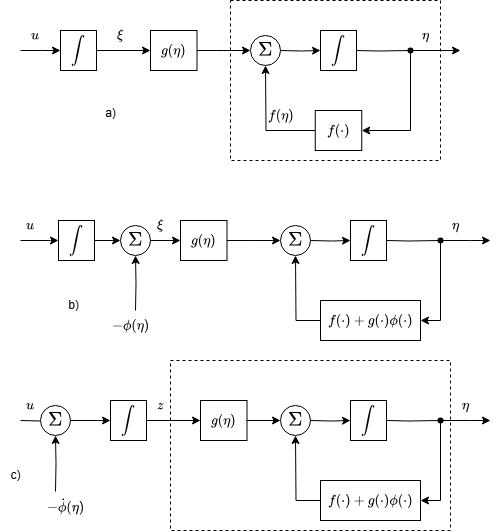
\includegraphics[width=0.48\textwidth]{Y1-report/Backstepping_diagram.drawio.png}
    \caption{Backstepping visualization block diagram series. a) Original system b) Introduce virtual control input c) Backstepping control input throught integrator}
    \label{fig:backstepping}
\end{figure}

\section{Proposed Methodology}
\subsection{Fault Detection and Diagnosis}
For the purposes of this paper, the FDI unit will not be implemented. Instead, the fault will be assumed to be perfectly known and injected directly into the system and the FTC unit will be used to reconfigure the controller. Mathematically the estimated fault can be incorporated into the control law as follows:
\begin{equation}\vec{u}=(\mathbf{I}_{n}-\mathbf{E})\vec{u}_{c}+\vec{u}_{a}\end{equation}

where $E$ represents the effecitve loss of actuators $E=diag(e_{1},e_{2}\dots,e_{n})$ and $0\leq e_{i}\leq 1$. $e_{i}=0$ means the actuator is healthy. Additionally $\vec{u}_{a}$ represents the additive bias fault.

%%%%%%%%%%%%%%%%%%%%%%%%%%%%%%%%%%%%%% FTC %%%%%%%%%%%%%%%%%%%%%%%%%%%%%%%%%%%%%%%%
\subsection{Fault Tolerant Control}
In this section, the steps used to obtain the control law from \cite{shenActiveFaulttolerantControl2019} are laid out. The kinematic equation can be re-written in the following form:


\begin{equation}\mathbf{J}\dot{\vec{\omega}_{b}}=-\mathbf{S}(\vec{\omega}_{b})\mathbf{J}\vec{\omega}_{b}+\mathbf{D}\vec{u}+\vec{d}\end{equation}

\begin{equation} \dot{\mathbf{Q}}=\frac{1}{2}\begin{bmatrix}
\mathbf{S}(\vec{q})+q_{0}\mathbf{I}_{3} \\
-\vec{q}^{T}
\end{bmatrix} \vec{\omega}_{b}\end{equation}
where $\mathbf{S}(x)$ represents the skew symmetric matrix, 
$\vec{q}=\begin{bmatrix}q_{1} \ q_{2} \ q_{3} \end{bmatrix}^T$ is the vector part of the spacecraft quaternion $\vec{Q}$,
$\vec{d}$ is the environmental disturbance torque,
$\vec{\omega}_{b}$ is the body angular velocity in body fixed frame and
$\mathbf{D}$ is the actuator configuration matrix.

\begin{equation}\vec{u}=(\mathbf{I}-\mathbf{E})\vec{u}_{c}+\vec{u}_{a}\end{equation}
where $E$ represents the effecitve loss of actuators $E=diag(e_{1},e_{2}\dots,e_{n})$ and $0\leq e_{i}\leq 1$. $e_{i}=0$ means the actuator is healthy. $\vec{u}_{a}$ additive bias fault.


\begin{equation}
    \mathbf{J}\dot{\vec{\omega}_{b}}=-\mathbf{S}(\vec{\omega}_{b})\mathbf{J}\vec{\omega}_{b}+\mathbf{D}\vec{u}_{c}+\vec{f}+\vec{d}
\end{equation} 
where $\vec{f}=\mathbf{D}\mathbf{E}\vec{u}_{c}+\mathbf{D}\vec{u}_{a}$ represents the influence of the fault on the system and acts as a disturbance on the system.



$\mathbf{D}^+=\mathbf{D}^T(\mathbf{D}\mathbf{D}^T)^{-1}$ is the pseudo inverse matrix

%%% Backstepping iteration 1 %%%
In \cite{shenActiveFaulttolerantControl2019} a non-linear virtual control input is chosen based on the paper by \cite{kimRobustBacksteppingControl2003}. This improves the torque profile and motion around the equilibrium point. The virtual control input is given by:

\begin{equation}\vec{\omega}_{c}=-\alpha\arctan(\beta\vec{q})\end{equation}

\begin{equation}\vec{s}=\vec{\omega_{b}}-\vec{\omega_{c}}=\vec{\omega_{b}}+\alpha\arctan(\beta\vec{q})\end{equation}

A Lyapunov function is chosen as 

\begin{equation}V_{1}=k_{0}\vec{q}^T\vec{q}+k_{0}(1-q_{0})^2\end{equation}

And it can be shown that 

% \begin{equation}\dot{V}_{1}\leq-k_{0}\alpha \lVert \vec{q} \rVert^{2}+k_0\alpha\vec{q}^T\vec{s}\end{equation}

% It's clear that $\dot{V}_{1}\leq0$ if $\vec{s}=0$ since $-k_{0}\alpha \lVert \vec{q} \rVert^{2}\leq0$.

\begin{equation}\dot{V}_{1}\leq-k_{0}\alpha \lVert \vec{q} \rVert^{2}\end{equation}

It's clear that $\dot{V}_{1}\leq0$ since $-k_{0}\alpha \lVert \vec{q} \rVert^{2}\leq0$.


%%% Backstepping iteration 2 %%%
We obtain the new kinematic equation in terms of $\vec{s}$ after substituting into (9):

\begin{equation}
    \begin{split}
        \mathbf{J}\dot{\vec{s}}&=
        \mathbf{J}\dot{\vec{\omega_b}} + \alpha\beta\mathbf{J}(\mathbf{I_3}+\beta^2\mathbf{\Xi}_q)^{-1}\vec{\dot{q}}\\
        &=-k_0\vec{q}+\mathbf{F}(\cdot)+\mathbf{D}\vec{u}_{c}+\vec{\hat{f}}+\vec{d}
    \end{split}
\end{equation}

where

\begin{multline}
    \mathbf{F}(\cdot)=k_0\vec{q}-\vec{\omega_b}^{\times}\mathbf{J}\vec{\omega_b}+\vec{\Delta f} + \vec{d} + \\
    \frac{1}{2}\alpha\beta\mathbf{J}(\mathbf{I}_3+\beta^2\mathbf{\Xi}_q)^{-1}(\mathbf{S}(\vec{q})+q_0\mathbf{I}_3)\mathbf{J}\vec{\omega}_{b}
\end{multline}

where $\Delta \vec{f}=\vec{f}-\vec{\hat{f}}$ is the bounded fault estimation error,
$\mathbf{\Xi}_q=diag(q_1^2,q_2^2,q_3^2)$ and
$\vec{\omega_b}^{\times}=\mathbf{S}(\vec{\omega_b})$. 
The control authority of the system changes significantly for the saturated and unsaturated actuator cases. Therefore a piecewise function must be defined which is continuous at the transition point. They define their control law as follows:

\begin{equation}
\vec{u}^{sat}_{c} = -\frac{u_{max}}{\epsilon_{0}}\mathbf{D}^+ sat[\Gamma(\cdot)\vec{s}]
\end{equation}
where $sat[\Gamma(\cdot)\vec{s}]$ is defined as

\begin{equation}
    sat[\Gamma(\cdot)\vec{s}]=\begin{cases}
        \frac{\vec{s}}{\lVert s \rVert} & \text{if } \lVert \vec{s} \rVert \geq \frac{u_{max}}{\epsilon_0\Gamma(\cdot)\vec{s}}\\
        \frac{\epsilon_0\Gamma(\cdot)\vec{s}}{u_{max}} & \text{if } \lVert \vec{s} \rVert \leq \frac{u_{max}}{\epsilon_0\Gamma(\cdot)\vec{s}}
    \end{cases}
\end{equation}

And 
\begin{equation}
\Gamma(\cdot)=k+\frac{\vec{s}^T\vec{\hat{f}}}{{\lVert \vec{s} \rVert}^2+\epsilon_{1}^2}+ 
\frac{\hat{h}\mathbf{\Omega}}{\lVert \vec{s} \rVert + \epsilon_{2}}
\end{equation}

Here $k$, $\epsilon_0$, $\epsilon_1$ and $\epsilon_2$ are constants, $\Omega = \lVert\vec{\omega}_b\rVert^2 + \lVert\vec{\omega}_b\rVert + 1$ $\hat{h}$ is defined as an adaptive law

%% Adaptive law
\begin{equation}
    \dot{\hat{h}} = -c_1\hat{h} + \frac{c_2\Omega\lVert\vec{s}\rVert^2}{\lVert\vec{s}\rVert+\epsilon_2}
\end{equation}
where $c_1$ and $c_2$ are positive constants.
Please see the Appendix \ref{apx:B} for proof of closed loop stability of this control law. 


\section{Results}
\subsection{Simulation Setup}
To demonstrate the effectiveness of the preceding algorithm from \cite{shenActiveFaulttolerantControl2019} A similar experimental set up is used as in \cite{shenActiveFaulttolerantControl2019} however here we look at the case where there is a total failure of an actuator to push the system to the limits. The moment of inertia is taken to be $\mathbf{J} = [10.0, 1.2, 0.5; 1.2, 19.0, 1.5;  0.5, 1.5, 25.0;]$. The disturbance torques as taken to be 
\newline $d(t) = [-0.005 sin(t), 0.005 sin(t), -0.005 sin(t)]^T \unit{Nm}$. Our fault is set as a complete failure of actuator 1, i.e.: \newline $e_1 = 0$ from $t_0$. Intial conditions are taken as 
$\omega_b(0) = \vec{0}$ and $\vec{Q}(0) = [-0.30481062, 0.0, 0.0, 0.95241298]^T$ with a final position of the identity quaternion which represents a 120 degree rotation in the direction on the failed actuator.  To compensate for the fault the following constant parameters are used in the controller: 
\newline $\alpha=0.2, \beta = 1.8, k = 100, \eta = 0.1, \upsilon = 0.01, c_1 = 0.01$ and the adaptive parameter $\hat{h}(0) = 0.1$. For the comparison case a quaternion feedback controller is simulated with the following control law chosen: $\vec{u}_c = -\mathbf{D}^+ (k_p \mathbf{J} \vec{q} + k_d \mathbf{J} \vec{\omega}_b)$ where kp and kd are chosen as 0.1422 and 0.533 respectively. The maximum torque is also limited to $\SI{0.2}{Nm}$ and the actuators speed is limited to 1000 rpm. The simulation is run for 300 seconds with a sampling time of 0.1 seconds. 
Plotted in figure \ref{fig:backstepping-results} and figure \ref{fig:q_feedback-results} are the results of the simulation. The first row shows the euler yaw, pitch and roll angles and the integral of the error angle about the euler axis of rotation(called euler integral here for brevity). From \cite{sidiAttitudeDynamicsKinematics1997}: the euler integral  "shows the overall angle path that the satellite traverses during the maneuver". It is calculated by taking $\int_{0}^{t} cos^{-1}(\frac{1}{2}[trace(\mathbf{A}_E)-1] dt$ where $A_E$ represents the error DCM. Row 2 shows the actuator control torques and the satellite angular rate.
%     \item $\mathbf{J} = \begin{bmatrix}
%         10.0 \ \ 1.2 \ \ 0.5 \\ 1.2 \ \ 19.0 \ \ 1.5 \\  0.5 \ \ 1.5 \ \ 25.0 \\
%     \end{bmatrix}  $
%     \item $\lVert u_{max} \rVert = 0.5 Nm$
%     \item 
% \end{itemize}
\begin{figure*}
    \centering
    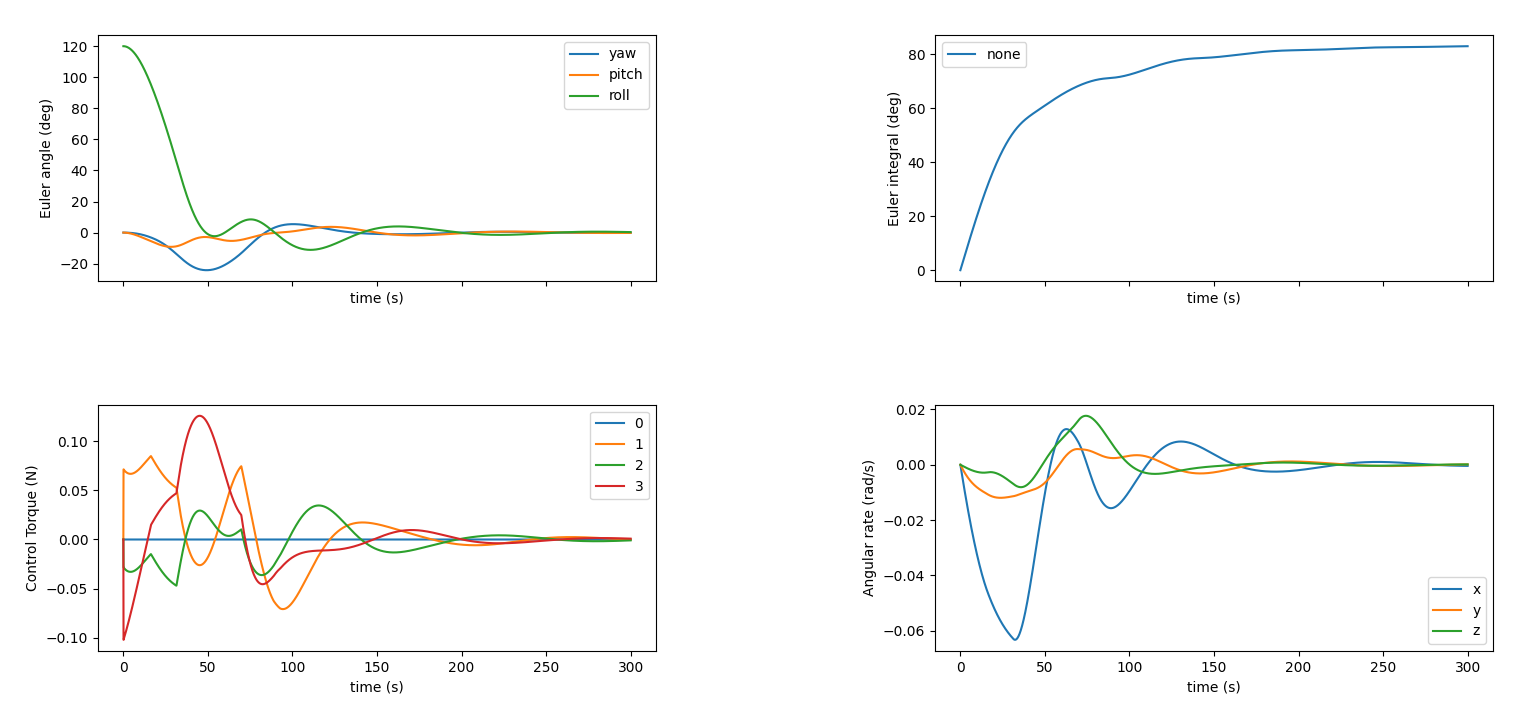
\includegraphics[width=\textwidth]{Y1-report/Results-q_feedback.png}
    \caption{Results showing the control performance of the quaternion feedback control with actuator failures and saturation. From left to right: the first row shows the euler yaw, pitch and roll angles and the integral of the error angle about the euler axis of rotation(called euler integral here for brevity). The second row shows the actuator control torques and the satellite angular rate.}
    \label{fig:q_feedback-results}
\end{figure*}
\begin{figure*}
    \centering
    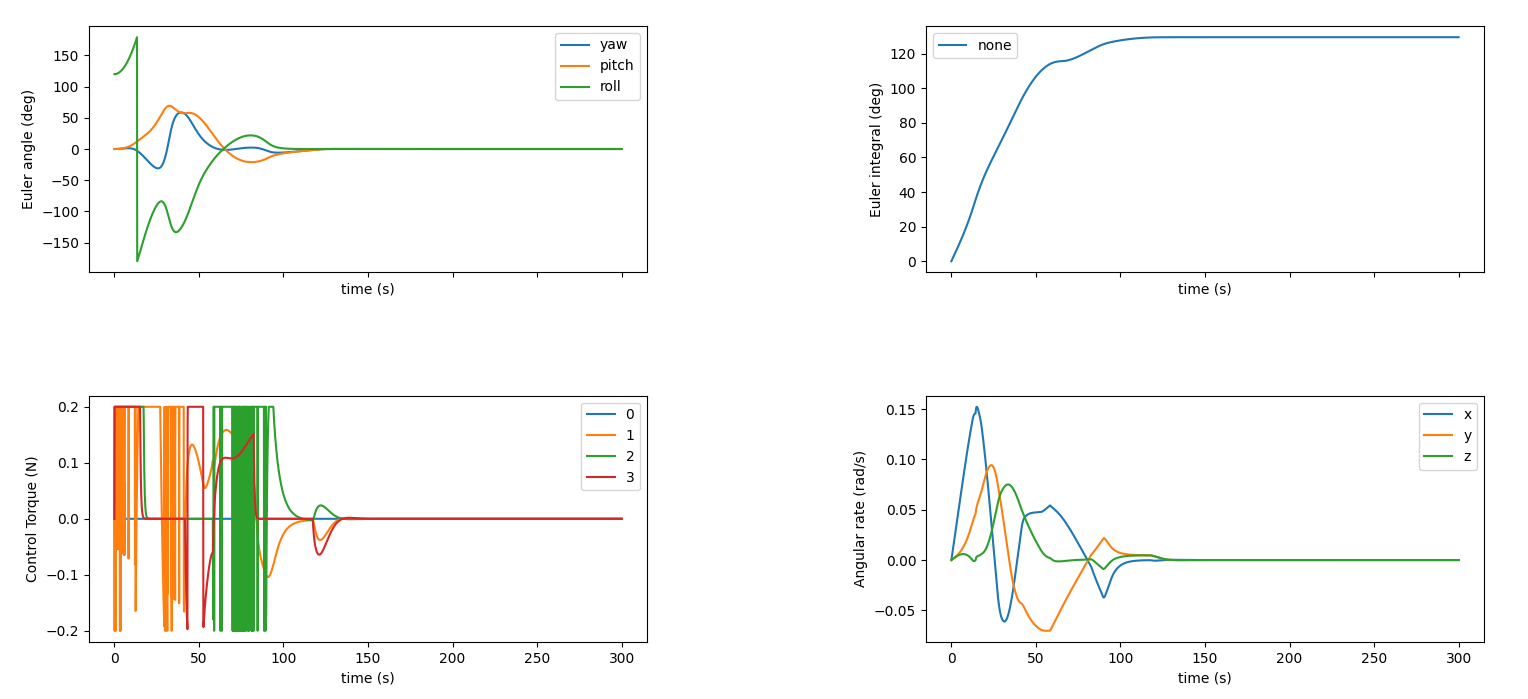
\includegraphics[width=\textwidth]{Y1-report/Results-backstepping_shen.png}
    \caption{Results showing the control performance of the backstepping controller with actuator failures and saturation. From left to right: the first row shows the euler yaw, pitch and roll angles and the integral of the error angle about the euler axis of rotation(called euler integral here for brevity). The second row shows the actuator control torques and the satellite angular rate.}
    \label{fig:backstepping-results}
\end{figure*}

\subsection{Analysis}
It is clear comparing the results in figure \ref{fig:backstepping-results} and figure \ref{fig:q_feedback-results} that the backstepping controller significantly improves performance. To give concreate numbers: the settling time improves from 283s to 115s and improves the pointing error from $\theta_e = [-0.1, -0.2, 0.3] deg (ypr)$  to $\theta_e = [\num{1.0e-10}, \num{1.33e-10}, \num{-1.86e-10}] deg (ypr)$. This is a major improvement and could allow a satellite to continue operations as normal.

\section{Appendix}
\subsection{}
Given the following Lyapunov function:
% \begin{equation}
%     V_{1}=k_{0}\vec{q}^T\vec{q}+k_{0}(1-q_{0})^2
% \end{equation}
$$
V_{1}=k_{0}\vec{q}^T\vec{q}+k_{0}(1-q_{0})^2
$$

\begin{equation}
    \begin{split}
    \dot{V_{1}}&=\frac{d}{dq}(k_{0}\vec{q}\cdot\vec{q}+k_{0}(1-q_{0})^2) \\
    &=\frac{d}{dq}(k_{0}\lVert\vec{q}\rVert^2+k_{0}(1-q_{0})^2) \\
    \end{split}
\end{equation}

from \cite{kimRobustBacksteppingControl2003} it is shown that

\begin{equation}
    \frac{d}{dq}(\lVert \vec{q} \rVert^{2}+(1-q_{0})^2) = \vec{q}^T \vec{\omega}
\end{equation}

and from the following lemma:

\begin{equation}
    -\alpha x \arctan(\beta x) \leq -\alpha x^2
\end{equation}

Thus
\begin{equation}
    \begin{split}
        \dot{V_{1}}&=k_{0}\vec{q}^T\vec{\omega_c} \\
        &= -\alpha k_{0}\vec{q}^T \arctan(\beta \vec{q}) \\
        &\leq -\alpha k_{0} \lVert\vec{q}\rVert^{2}
    \end{split}
\end{equation}

\subsection{} \label{apx:B}
\subsubsection{Case 1} $\lVert \vec{s} \rVert \geq \frac{u_{max}}{\epsilon_0\Gamma(\cdot)\vec{s}}$
\begin{equation}
\vec{u}_c^{sat} = -\frac{u_{max}}{\epsilon_0}\mathbf{D}^+ \frac{\vec{s}}{\lVert \vec{s} \rVert}
\end{equation}

For the first case (no actuator saturation) the following candidate Lyapunov function is chosen (similar to the previous section on backstepping):

\begin{equation}
    V_2=V_1 + \frac{1}{2}\vec{s}^T\mathbf{J}\vec{s}
\end{equation}

Taking the derivative and substituting in we get:

\begin{equation}
    \begin{split}
        \dot{V_2} &= k_0\vec{\omega_b}^T\vec{q} + k_0\vec{q}^T\vec{s} + \vec{s}^T(-k_0\vec{q} + \mathbf{F}(\cdot) + \mathbf{D}\vec{u}_c^{sat} + f) \\
        &=  k_0\vec{\omega_b}^T\vec{q} + \vec{s}^T(\mathbf{F}(\cdot) + \mathbf{D}(-\frac{u_{max}}{\epsilon_0}\mathbf{D}^+ \frac{\vec{s}}{\lVert \vec{s} \rVert}) + f) \\
    \end{split}
\end{equation}

Now we show that

\begin{equation}
    \lVert\mathbf{F}(\cdot)\rVert \leq \bar{J}\lVert\vec{\omega}_b\rVert^2 + \frac{1}{2}\alpha\beta\lVert\vec{\omega}_b\rVert + k_0 + \delta + \bar{d}	\leq h\Omega 
\end{equation}

follows from the assumptions:
\paragraph{Assumption 1} $\underline{J} \leq \lVert\vec{J}\rVert \leq \bar{J}$ where $\underline{J}$ and $\bar{J}$ are positive constants.

\paragraph{Assumption 2} Environmental disturbances due to gravitation, solar radiation pressure, magnetic forces, or aerodynamic forces are bounded by positive constant $\bar{d}$ such that $\lVert\vec{d}\rVert \leq \bar{d}$.

\begin{equation}
    \lVert\vec{\omega}_b^\times\mathbf{J}\vec{\omega}_b \rVert \leq \bar{J}\left\lVert\vec{\omega}_b\right\rVert 
\end{equation}
\begin{equation}
    \left\lVert k_0\vec{q} + \vec{\Delta f} + \vec{d} \leq k_0 + \delta + \bar{d}\right\rVert \label{eq:apx}
\end{equation}
\begin{equation}
    \left\lVert\frac{1}{2}\alpha\beta\mathbf{J}(\mathbf{I}_3 + \beta^2\mathbf{\Xi}_q)^{-1}(\mathbf{S}(\vec{q}) + q_0\mathbf{I}_3)\vec{\omega}_b\right\rVert \leq \frac{1}{2}\alpha\beta\bar{J}\left\lVert\vec{\omega}_b\right\rVert 
\end{equation}
from the fact that $-1 \leq q_0,q_1,q_2,q_3 \leq 1$ we know that $\left\lVert(\mathbf{S}(\vec{q}) + q_0\mathbf{I}_3)\right\rVert  \leq 1$\footnote{see proof below (TBD)} and $\left\lVert(\mathbf{I}_3+\beta^2\mathbf{\Xi})^{-1}\right\rVert  \leq 1$. Thus we can conclude that 
\begin{equation}
    \lVert\mathbf{F}(\cdot)\rVert \leq \bar{J}\lVert\vec{\omega}_b\rVert^2 + \frac{1}{2}\alpha\beta\lVert\vec{\omega}_b\rVert + k_0 + \delta + \bar{d}	\leq h\Omega
\end{equation}

where $\Omega = \lVert\vec{\omega}_b\rVert^2 + \lVert\vec{\omega}_b\rVert + 1$ and $h=max\{\bar{J},\frac{1}{2}\alpha\beta\bar{J},k_0 + \delta + \bar{d}\}$

Note that \ref{eq:apx} is a result of the assumption that estimation errors are bounded after successful fault identification: $\lVert\vec{\Delta f}\rVert \leq \delta$ where $\delta$ is a positive constant.

Therefore 
\begin{equation}
    \dot{V}_2 \leq -k_0\alpha\lVert \vec{q} \rVert^2 + \lVert \vec{s} \rVert\mathbf{D}^+\vec{u}_{sat} + \lVert \vec{s} \rVert h \Omega + \lVert \vec{\hat{f}} \rVert\lVert \vec{s} \rVert
\end{equation}

They assume that $\frac{u_{max}}{\epsilon_0} \geq h\Omega + \lVert \vec{\hat{f}} \rVert + \varrho_0$ where $\varrho_0$ is a small constant. substituing in and rearranging gives us:

\begin{equation}
    \dot{V}_2 \leq -k_0\alpha\lVert \vec{q} \rVert^2 - \varrho_0\lVert \vec{s} \rVert \leq 0
\end{equation}
\subsubsection{Case 2} $\lVert \vec{s} \rVert \leq \frac{u_{max}}{\epsilon_0\Gamma(\cdot)\vec{s}}$
They choose a different Lyapunov function for this case as:
\begin{equation}
    V_2=V_1+\frac{1}{2}\vec{s}^T\mathbf{J}\vec{s} + \frac{1}{2c_2}\tilde{h}^2
\end{equation}
and after a more complicated procedure (but with the same fundementals) obtain the following control law:
\begin{equation}
    \vec{u}_c^{sat} = \mathbf{D}^+ \Gamma(\cdot) \vec{s}
\end{equation}